% ********** Rozdział 2 **********
\chapter{Opis struktury projektu}
Projekt wykonany został w języku C\# z wykorzystaniem .NET 8.0, dodatkowo baza danych opiera się na SQL, integrację bazy danych z aplikacją ułatwiło wykorzystanie biblioteki Microsoft.Data-SqlClient w wersji 5.2.2, kolejnym narzędziem wykorzystanym do projetku jes CsvHelper.

\noindent \textbf{Minimalne wymagania sprzętowe do projektu to:}
\begin{itemize}
    \item Procesor: Intel Core i5 lub wyższy.
    \item Pamięć RAM: 8 GB.
    \item Dysk: Co najmniej 10 GB wolnego miejsca.
\end{itemize}

\noindent \textbf{Zarządzanie bazą danych:}
Aplikacja wykonuje operacje CRUD dzięki którym możemy dynamicznie działać pomiędzy bazą danych a aplikacją, największy dostęp do bazy ma pracownik z dostępem administratora, ponieważ może dodawać, usuwać jak również i aktualizować zamówienia, może również eksportować i importować dane z plików csv aby wybrać pracownika miesiąca.

Klient jak i kurier mają dostęp do nadawania i odbierania paczek do których mają dostęp jak również wyświetlenia informacji o swoim profilu i liście paczek przypisanych do danego użytkownika.

\noindent \textbf{Hierarchia klas w projekcie:}

\begin{figure}[h!]
    \centering
    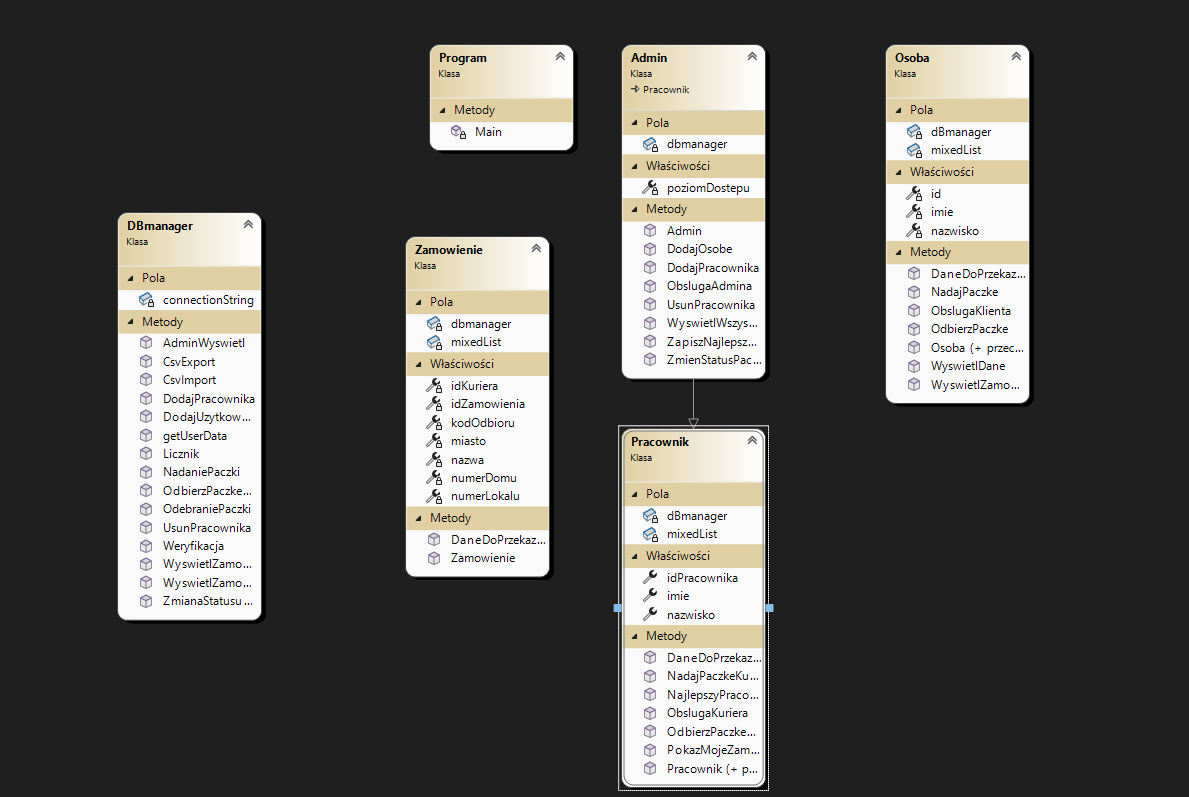
\includegraphics[width=0.8\textwidth]{diagram klas.png}
    \caption{Diagram przedstawiający hierarchię klas w projekcie.}
\end{figure}

Klasy zostały utworzone dla potrzeb projektu z myślą o podziale na klientów i pracowników, klasa pracownik jest klasą przewidzianą dla kurierów bez dostępu do trybu administratora, używa metod z klasy DBManager, jest to klasa stworzona do obslugi działań crudowych z bazą danych, to w niej znajdują się najważniejsze metody takie jak wyświetlanie wszystkich zamówien, zmiana status zamówienia, usuwania i dodawanie użytkowników, klasa pracownik czerpie z dbManagera poprzez dodawanie dancych klasy Pracownik do bazy danych, klasa Admin dziedziczy z klasy Pracownik rozszerzajac ją o poziom dostępu, jest to właściwość definiująca czy dany kurier ma dostęp do trybu administratora, metody admina to wszystkie operacje CRUD na bazie dlatego ważna jest weryfikacja poziomu dostępu, admin może również tworzyć plik CSV wykorzystywany do określenia najlepszego pracownika miesiąca. Klasa osoba jest klasą przypisaną klientom, mają możliwość nadawania i odbierania swoich paczek jak również wyświetlanie swoich danych i zamówień
przypisanych im w paczkomacie. Klasa Zamówienie jest klasą obsługującą nadawanie zamówień przez inne klasy, zwaraca one dane do zamówienia które poźniej zostają przekazane do naszej bazy danych.